
\chapter{Chess playing AI}\label{sec:topic-analysis}
Before further discussion about thesis topic, it is require to analyze main components and issues related to it. To make those speculations easier to understand and internalize, they will be divided into two main sections: chess game logic and application logic. Both of those topics will be described in each distinct sections, starting with chess game logic.
    \section{Chess}
    Chess is a board game in which two players compete against each others by using 16 chess pieces \cite{bib:book-chess-bible}. Each game is started by white site player an after that both players performs their actions sequentially, one by one. There are three ways to end the game. First option is to left enemy king piece without any moves. This manoeuver is called \textbf{checkmate}. One more thing that needs to be achieved to perform checkmate is to put enemy king in the \textbf{check} situation (threatened with capture by enemy piece) \cite{bib:book-chess-bible,bib:internet-learn-how-to-play-chess}. 

    Second method to end the game is to wait until time will end. Standard time limit used on a lot of major chess tournaments is 90 min. That means that both players have 90 minutes to finish game. When time will end and player still performing his move, he loses the game. Usage of the time limit force players to thing and act fast but still according to their game plan.

    Last option to end chess game is to force enemy player to resign. In that case, situation is simple and player who resigned, loses the game. 
    
    As it was mentioned before, every player need to use their 16 chess pieces and adapt the strategy to make opponent lose. In the \hyperref[tab:chess-pieces-list]{tab. \ref*{tab:chess-pieces-list}} are shown all chess pieces types with their unique move patterns and special properties. Quick remark: in the table, pieces are not differentiate by its color because either white and black piece work the same way. Mentioned chess pieces are deployed on the chess board of dimensions $8 \times 8$ (as it is shown on \hyperref[fig:beginning-chessboard-layout]{fig. \ref*{fig:beginning-chessboard-layout}}), then the game starts by white site player move \cite{bib:book-chess-bible,bib:book-bobby-fisher-teaches-chess,bib:book-mastering-chess-logic}.

    \begin{table}
        \centering
        \caption{The list of chess pieces.}
        \label{tab:chess-pieces-list}
        \begin{tabular}{ccp{0.4\textwidth}p{0.3\textwidth}}
        \toprule
            \textbf{symbol} & \textbf{name} & \textbf{moving pattern} & \textbf{special properties}\\
            \hline
                \WhiteKingOnWhite \BlackKingOnWhite & king & rectilinear or diagonal movement, only by one square & castling\\
            \hline
                \WhiteQueenOnWhite \BlackQueenOnWhite & queen & rectilinear or diagonal movement, over any number of squares & none\\
            \hline
                \WhiteBishopOnWhite \BlackBishopOnWhite & bishop & diagonal movement, over any number of squares & none\\
            \hline
                \WhiteKnightOnWhite \BlackKnightOnWhite & knight & rectilinear movement, by one square, then diagonal movement in the same direction, by one square & jumping over other pieces\\
            \hline
                \WhiteRookOnWhite \BlackRookOnWhite & rook & rectilinear movement, over any number of squares & castling\\
            \hline
                \WhitePawnOnWhite \BlackPawnOnWhite & pawn & move forward, by one square or diagonal movement by one square while capturing & promotion, \french{en passant}, in case of first move can move by one or 2 squares forward\\
        \end{tabular}
    \end{table}

    \begin{figure}
        \centering
        \newgame
        \showboard
        \caption{Chessboard layout at the beginning of the game.}
        \label{fig:beginning-chessboard-layout}
    \end{figure}

    \begin{description}
        \item[Castling] is an manoeuver which includes king piece and on of the rooks. It consist in moving king horizontally, by two squares, towards the participating rook and then placing rook on square which was passed by king. Requirements to perform castling manoeuver:
        \begin{itemize}
            \item both pieces needs to be in the same color,
            \item castling needs to be first move performed by both pieces in this game,
            \item squares between both pieces needs to be blank and not attacked by enemy pieces,
            \item king cannot be under check and performing castling manoeuver cannot result in this situation.
        \end{itemize}
        There are two types of castling (short castling and long castling) which are presented on \hyperref[fig:castling-manoeuver]{fig. \ref*{fig:castling-manoeuver}}. In the past there were third type of castling which has been performing by rook created by promotion manoeuver. Unfortunately, this manoeuver has been outlawed in 1972.

        \begin{figure}
            \centering
            \newchessgame[setwhite={ke1, rh1}, addblack={ke8, ra8}]
            \hidemoves{1. O-O O-O-O}
            \chessboard[moveid=1w, pgfstyle=straightmove, color=blue,
                        markmoves=\xskakget{move}, color=red, markstyle=circle, 
                        markfield=\xskakget{movefrom}, emphfields=\xskakget{moveto},
                        moveid=1b, pgfstyle=straightmove, color=blue,
                        markmoves=\xskakget{move}, color=red, markstyle=circle, 
                        markfield=\xskakget{movefrom}, emphfields=\xskakget{moveto}]
            \caption{Castling manoeuver (short castling on white site, long castling on black site).}
            \label{fig:castling-manoeuver}
        \end{figure}

        \item[Jumping over other pieces] is an manoeuver which can be performed only by knight piece. It consist in moving knight piece on the destination square even if path is blocked by other piece. Jumping manoeuver is presented on \hyperref[fig:jumping-manoeuver]{fig. \ref*{fig:jumping-manoeuver}}.
        
        \begin{figure}
            \centering
            \newchessgame
            \hidemoves{1. Nf3 Na6}
            \chessboard[moveid=1w, pgfstyle=curvemove, color=blue,
                        markmoves=\xskakget{move}, color=red, markstyle=circle, 
                        markfield=\xskakget{movefrom}, emphfields=\xskakget{moveto},
                        moveid=1b, pgfstyle=curvemove, color=blue,
                        markmoves=\xskakget{move}, color=red, markstyle=circle, 
                        markfield=\xskakget{movefrom}, emphfields=\xskakget{moveto}]
            \caption{Jumping manoeuver.}
            \label{fig:jumping-manoeuver}
        \end{figure}

        \item[Promotion] in an specific manoeuver which can be performed only by pawn piece. It happens when one of pawns reach enemy site of the chessboard. In that situation player chooses any piece of the same color (except king) on which he want to replace pawn which performed promotion. This manoeuver allows for situation in which, for example there will be more than 1 queen in the same game. Promotion manoeuver is presented on \hyperref[fig:promotion-manoeuver]{fig. \ref*{fig:promotion-manoeuver}}.
        
        \begin{figure}
            \centering
            \begin{subfigure}{\textwidth}
                \centering
                \newchessgame[setwhite={ke1, pa7}, addblack={ke8, ph2}]
                \hidemoves{1. a8 h1}
                \chessboard[moveid=1w, pgfstyle=straightmove, color=blue,
                            markmoves=\xskakget{move}, color=red, markstyle=circle, 
                            markfield=\xskakget{movefrom}, emphfields=\xskakget{moveto},
                            moveid=1b, pgfstyle=straightmove, color=blue,
                            markmoves=\xskakget{move}, color=red, markstyle=circle, 
                            markfield=\xskakget{movefrom}, emphfields=\xskakget{moveto}]        
                \hfill
                \newchessgame[setwhite={ke1, pa7}, addblack={ke8, ph2}]
                \hidemoves{1. a8=Q h1=B}
                \chessboard[moveid=1w, pgfstyle=straightmove, color=blue,
                            markmoves=\xskakget{move}, color=red, markstyle=circle, 
                            markfield=\xskakget{movefrom}, emphfields=\xskakget{moveto},
                            moveid=1b, pgfstyle=straightmove, color=blue,
                            markmoves=\xskakget{move}, color=red, markstyle=circle, 
                            markfield=\xskakget{movefrom}, emphfields=\xskakget{moveto}]
            \end{subfigure}
            \caption{Promotion manoeuver (white pawn from square a7 promoted to queen, black pawn from square h2 promoted to bishop).}
            \label{fig:promotion-manoeuver}
        \end{figure}

        \item[\french{En Passant}] is an special variant of capturing, assigned to pawn piece. This capturing can be performed if enemy pawn made move by two squares and crossed square that is attacked by performing pawn. In that situation, capturing pawn is moved on attacking square and enemy pawn gets removed from chessboard. One last requirements to perform \french{en passant} is to perform it directly after enemy pawn move. \french{En Passant} manoeuver is presented on \hyperref[fig:en-passant-manoeuver]{fig. \ref*{fig:en-passant-manoeuver}}.
        
        \begin{figure}
            \centering
            \begin{subfigure}{\textwidth}
                \centering
                \newchessgame[setwhite={ke1, pd2}, addblack={ke8, pe4}]
                \hidemoves{1. d4}
                \chessboard[pgfstyle=straightmove, color=blue,
                            markmoves=\xskakget{move}, color=red, markstyle=circle, 
                            markfield=\xskakget{movefrom}, emphfields=\xskakget{moveto}]        
                \hfill
                \newchessgame[setwhite={ke1, pd2}, addblack={ke8, pe4}]
                \hidemoves{1. d4 exd3}
                \chessboard[moveid=1w, pgfstyle=straightmove, color=blue,
                            markmoves=\xskakget{move}, color=red, markstyle=circle, 
                            markfield=\xskakget{movefrom}, emphfields=\xskakget{moveto},
                            moveid=1b, pgfstyle=straightmove, color=blue,
                            markmoves=\xskakget{move}, color=red, markstyle=circle, 
                            markfield=\xskakget{movefrom}, emphfields=\xskakget{moveto}]
            \end{subfigure}
            \caption{\french{En Passant} manoeuver.}
            \label{fig:en-passant-manoeuver}
        \end{figure}
    \end{description}

    That is all of the chess game rules. At the beginning, chess may seem like very easy game but it happens to be very difficult problem ro be resolved by machine. Even thou, it is hard to ,,teach'' machine to play chess, there are a lot of chess engines which realize this functionality \cite{bib:article-impact-of-artificial-intelligence-on-chess-world}. The most known chess playing softwares are: ,,AlphaZero'' created by Google company \cite{bib:internet-alphazero,bib:article-chessai-in-game-analysis}, ,,Stockfish'' created by Marco Costalba, Tord Romstad and Joona Kiiski \cite{bib:article-chessai-in-game-analysis,bib:article-competing-paradigms-for-machine-intelligence} and ,,Leela Chess Zero (Lc0)'' created by Gary Linscott and Alexander Lyashuk.
    
    \section{Game trees}
    After describing problem that needs to be solved, it is necessary to describe solution to the problem. There is no analytic solution for the chess game so for solving this problem comprehensive approach is mostly used. Core element in all, previously mentioned chess playing softwares, is a game tree. Game tree is a graph data structure which consists of all possible moves that players can make. It is safe to say that usage of game tree is the most efficient algorithm which allows machine to make decisions. A lot of chess playing softwares uses this methodology with great success \cite{bib:internet-alphazero,bib:article-competing-paradigms-for-machine-intelligence,bib:article-chessai-in-game-analysis}.

    Game tree consists of two main components:
    \begin{description}
        \item[Node] is an representation of situation on the chessboard. Each node is created on proper tree level which reflect particular player turn.
        \item[Branch] represent each move that player can make in particular situation.
    \end{description}
    Game tree structure have one last property which is \textbf{game complexity}. This property is an number of nodes in last layer of complete game tree \cite{bib:article-impact-of-artificial-intelligence-on-chess-world}.
    
    To simplify further description of this issue, instead of using chess as an example, easier game called ,,Hexapawn'' will be used. It is a board game based on chess but its rules are much more simple. Each player have 3 pawns (functioning in the same way like pawns in chess), on the opposite sites of $3 \times 3$ board. Player can win by one of 3 ways:
    \begin{itemize}
        \item reach enemy site of the board with one of the pawns,
        \item capture all of enemy pawns,
        \item leave opponent with no moves.
    \end{itemize}
    Hexapawn was created by american mathematician Martin Gardner in March 1962 \cite{bib:article-hexapawn}. Hexapawn has been created to demonstrate first AI machine. This game fits perfectly for this usage because of its relatively small game tree. For the purpure of this thesis, Hexapawn has been simplified to just 2 pawns for each player and board of dimensions $2 \times 3$. Rest of the rules, mentioned before, are unchanged.

    \subsection{Game tree building process}\label{sec:game-tree-building-process}
    Due to the relatively low degree of complexity, previously mentioned game will be used as an example in game tree building process. As in all tree based graphs, building process starts from \textbf{root node} which is a first node that will be basis of the entire structure. After generating root node, next level of nodes is generated and attached to root node. Process of generating entire tree level base on actual situation on the board. In that case number of nodes in the layer depends on number of moves that player can perform in given situation. After first level of the game tree has been generated, the same process is applied to further levels. It is important to remember that players performs their moves alternately, which mean next generated tree level will be generated with second player point of view. Completely generated game tree for used version of Hexapawn is presented on \hyperref[fig:complete-game-tree-hexapawn]{fig. \ref*{fig:complete-game-tree-hexapawn}}.
    \begin{figure}
        \centering
        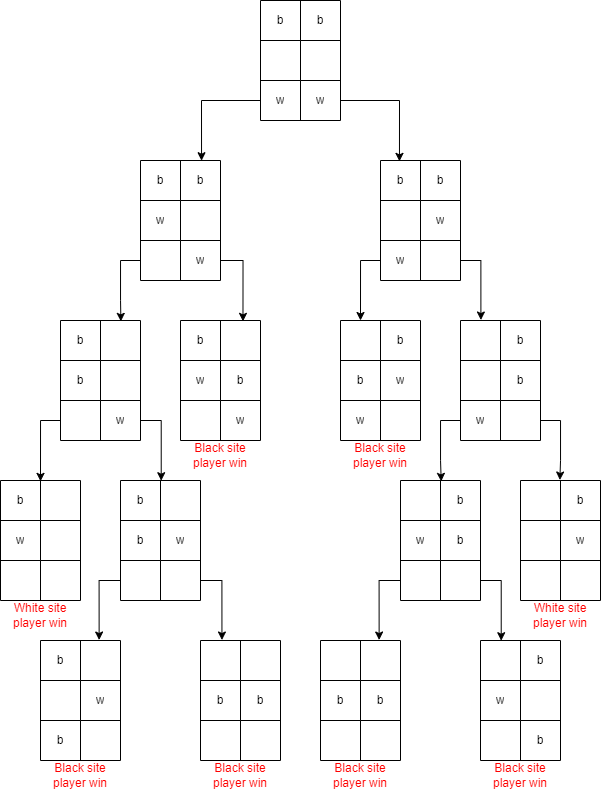
\includegraphics[width=\textwidth]{dependencies/pictures/Complete_Game_Tree.png}
        \caption{Complete game tree for simplified Hexapawn (w - white pawns, b - black pawns).}
        \label{fig:complete-game-tree-hexapawn}
    \end{figure}
    Last thing worth mentioning is the the fact that each game tree node consists not only from representation of chessboard, but also from evaluation value which has been assigned to this situation. However, this is a topic related directly to the functional aspect of the game tree which will be further discussed in section \ref{sec:min-max-algorithm}.

    \subsection{Min-max algorithm}\label{sec:min-max-algorithm}
    Even if game trees are crucial components while constructing AI, this component won't allow created instance for making decisions. To make those kind of operations \textbf{min-max tree} can be used. This structure i basically a game tree but every tree node consists also from evaluation value. Second difference between game tree and min-max tree is the fact that in second structure uses search algorithm called \textbf{min-max algorithm}. Before describing how min-max algorithm works it is important to explain how to evaluate each tree node. To calculate evaluation value for each nodes in the game tree evaluation functions are used. This type of function take as an input content of the tree node and return evaluation that needs to be assign to this node. More about evaluation functions in scope of this thesis can be found in section \ref{sec:game-tree-optimizations}.

    To explain how min-max algorithm works, generated game tree from \hyperref[fig:complete-game-tree-hexapawn]{fig. \ref*{fig:complete-game-tree-hexapawn}} will be used. Because generated tree present whole game (it is possible to see all outcomes), very simple evaluation function has been used. If given node resulted in white site player win, evaluation will be equal to $1$. Otherwise, evaluation will be equal to $-1$. The calculated values were assigned to proper nodes as it is presented on \hyperref[fig:min-max-tree-hexapawn]{fig. \ref*{fig:min-max-tree-hexapawn}}.
    \begin{figure}
        \centering
        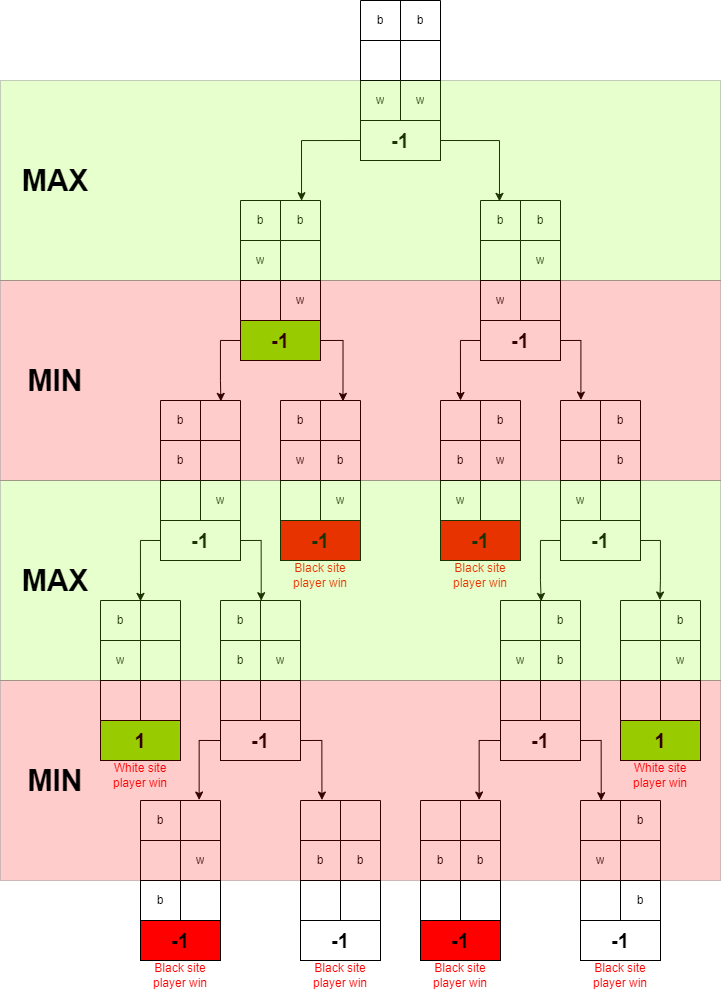
\includegraphics[width=0.8\textwidth]{dependencies/pictures/MinMax_Example.png}
        \caption{Min-max tree for simplified Hexapawn.}
        \label{fig:min-max-tree-hexapawn}
    \end{figure}

    As it can be seen on \hyperref[fig:min-max-tree-hexapawn]{fig. \ref*{fig:min-max-tree-hexapawn}}, it present also usage of min-max algorithm which will be now described.

    Structure analysis begins from is leafs. In the first iteration two nodes containing values $-1$ and $-1$ are compared. Because this layer represent opponent move, node with the lowest value got chosen (marked with red color). It happens because by definition, the opponent will make optimal moves, leading to a favorable situation for him. In the given situation, when both values are equal, first encountered value get chosen. After node comparison, chosen value is moved to node above for further comparisons. The same actions has been performed for rest nodes in this layer. After all nodes in last layer get compared, layer above needs to be analyze next. In case of this layer, comparing process is similar to te previous layer. Because analyzing layer represent AI move, among comparing nodes, the one with the highest value gets chosen (from both first nodes, value $1$ gets chosen and marked with green color). Similar like in last layer all chosen values are moved to layer above for further comparisons. By using this workflow, all root nodes evaluations needs to be calculated. Situation presented on \hyperref[fig:min-max-tree-hexapawn]{fig. \ref*{fig:min-max-tree-hexapawn}} shows that both root nodes have the same evaluation value so first encountered value get chosen \cite{bib:article-comparizon-of-search-algorithms}.

    \subsection{Game tree optimizations}\label{sec:game-tree-optimizations}
    Simplify version of game Hexapawn is simple enough it is possible to generate full game tree (resolve the game). Unfortunately, game that is a topic of this thesis is much more complex which means, resolving chess game is unreachable. Basing on average branching factor for chess game $b \approx 35$, and average game length $m \approx 70$, Victor Allis estimate complexity of the average game of chess to be $10^{123}$ \cite{bib:book-search-for-solutions-in-games}. That big complexity is potentially problematic because of big memorial and computational complexity of entire structure. Because of this complexity, a common practice is optimizing game tree size \cite{bib:article-optimal-on-game-trees}.

    The most commonly used optimization method is limiting depth of generating structure. In a lot of chess playing softwares, algorithm that generate game tree, do it until some constant value (most commonly this value is $3$) \cite{bib:internet-alphazero,bib:book-search-for-solutions-in-games,bib:article-optimal-on-game-trees}. This solution determine how many moves can be handled by created structure but prevents from solving the game. Usage of this optimization method force to use evaluation method because by analyzing only fragment of the game tree it is impossible to know all outcomes. There are multiple approaches to creating evaluation function. The simplest solution is to use heuristic equations \cite{bib:conference-heuristic-evaluation-chessai}. In this thesis evaluation will be handled by more complex solution, which is implemented and trained neural network instance. Used solution will be further described in section \ref{sec:neural-networks}. There are much more optimization methods that can be used, like $\alpha$-$\beta$ pruning, but in scope of this thesis, only game tree depth limitation has been used. 


    \section{Neural networks}\label{sec:neural-networks}
    As it was mentioned before, evaluation values that will be used in generated game tree, will be provided by neural network instance. While analyzing the problem it turned out that there are two types of neural network which can work with good effectiveness. As a scope of this thesis is to test which one of those two types of neural networks is more suitable for given problem of chess game. Two neural networks that will be described are Artificial Neural Network (ANN) and Convolutional Neural Network (CNN).

    \subsection{Artificial neural network}\label{sec:artificial-neural-network}
    To simplify further descriptions, it is better to start with ANN topic as it is the simplest version of any neural networks. Neural network is and mathematical structure model which uses basic processing elements (neurons) to perform some kind of operation on input data. An inspiration for this model is real-life neural systems. There are a lot of different types of neural networks but all of them consists of 2 main components: neuron and weight \cite{bib:internet-neural-network-and-deep-learning}. To avoid misunderstanding, in the further part of this thesis, both ,,artificial neural network'' and ,,neural network'' will relate to the same type of neural network. Artificial neural network in its most basic form can consists of following elements:
    \begin{description}
        \item[Weight] represent the connection between neurons. Each weight have also value assign to it which represent how strong particular connection is. Weights values are first of parameters that are modified in learning process. Learning process for ANN will be further described in this section (\ref{sec:learning-process-for-nn-instance}).
        \item[Neuron] is the most basic element of neural network. It is element performing mathematical operation on input data and as an output it return just single value. Output value of neuron $k$ in layer $m$ ($n_k^{(m)}$) can be calculated using following equation:
        \begin{equation}\label{eq:ann-neuron-value}
            n_k^{(m)} = f\left(b_i + \sum_{i = 0}^{l} w_{m-1, i} n_i^{(m-1)}\right),
        \end{equation}
        where:
        \begin{itemize}[label=]
            \item $n_i^{(m-1)}$ -- output value of neuron $i$ in layer $(m-1)$, $w_{m-1, i}$ -- weight value from neuron $i$ in layer $(m-1)$, $b_i$ -- value of bias $i$, $l$ -- number of neurons in layer $(m-1)$, $f$ -- activation function.
        \end{itemize}
        As it can be seen in equation \eqref{eq:ann-neuron-value} activation function was used. In this thesis, for artificial neural network, sigmoid function has been used ($a=\frac{1}{1 + e^{-n}}$). This activation function squash input value in range $(0, 1)$ but another, often used range o this function is $(-1, 1)$ \cite{bib:internet-sigmoid-function}. In case of this thesis, second range has been used.
        \item[Layer] works as and organization unit for neurons which define in which order, those neurons will be processed. Usually, artificial neural network consists of 3 types of layer \cite{bib:book-make-own-neural-network}:
        \begin{itemize}
            \item Input layer -- represent group of neurons containing input data. Neurons in this layer do not have weights and their value are not passed through activation function.
            \item Hidden layer -- represent group of neurons which are located between first and last layer of the network. Number of hidden layers and number of their neurons are not strictly defined and often it needs to be experimented with, to find the best setup for given problem.
            \item Output layer -- represent group of neurons located at the end of the network which is also network answer for given problem.
        \end{itemize}
        \item[Bias] is a additional neuron in each layer which is used for output regulations. This neuron also have weight value, that is why this weight value can be skipped in output calculations. Value of the bias is added to final sum of neuron values and their weights as it has been shown in equation \ref{eq:ann-neuron-value}. Value of the bias is the second modifiable parameters, changed in learning process.
    \end{description}
    For better understanding of neural network structure, on \hyperref[fig:ann-example]{fig. \ref*{fig:ann-example}} has been shown simple example of this kind of network. As it can be seen, this network consists of 3 layers (1 input layer, 1 hidden layer and 1 output layer) and value from input layer gets propagated through all other layers.
    \begin{figure}
        \centering
        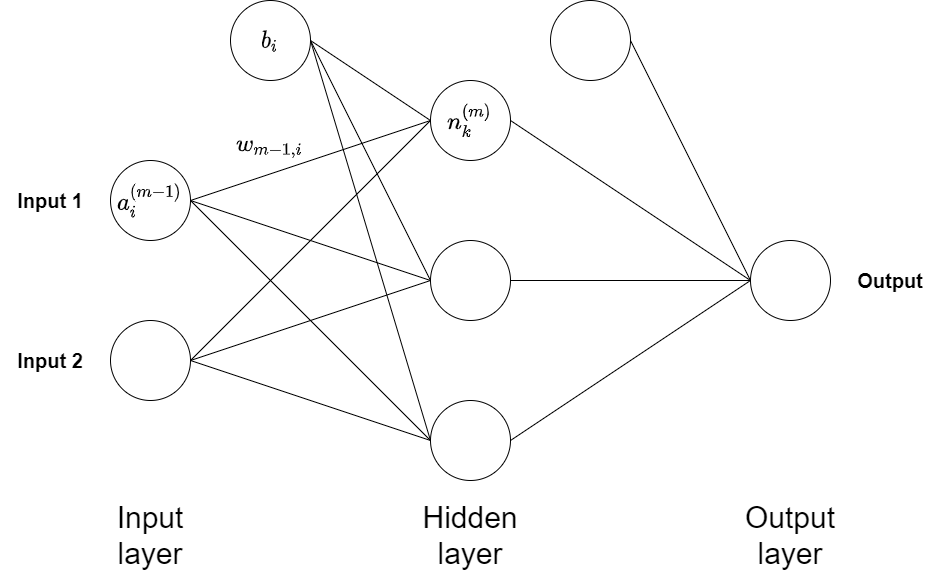
\includegraphics[width=0.8\textwidth]{dependencies/pictures/NN_example.png}
        \caption{Artificial neural network example.}
        \label{fig:ann-example}
    \end{figure}
    Process shown of \hyperref[fig:ann-example]{fig. \ref*{fig:ann-example}} is called \textbf{feed forward algorithm} and constitute whole process of resolving problems in neural networks. Feed forward process begins from loading input data into input layer. Then, by using equation presented in \ref{eq:ann-neuron-value}, those values are propagated through all hidden layers (if their exist) and lastly, final answer can be seen in output layer \cite{bib:book-make-own-neural-network,bib:article-application-of-feedforward-for-grade-estimation,bib:internet-neural-network-and-deep-learning}. It was decided to use this type of neural network, for chess game problem, because it is the most basic type of neural network so it will be very good comparison point for other used models.

    \subsection{Convolutional neural network}
    As it was mentioned before, scope of this thesis is to compare two neural network models and decide which one performs better in case of chess game problem. Second type of neural network that will be used for this task is Convolutional Neural Network. Why this type of network? Convolutional neural networks (CNN) act as pattern detecting algorithm. The most common usages of this model are: cancer detection, picture classifications, face detection, recognizing hand-written digits etc. \cite{bib:internet-real-world-applications-of-cnn}. Because of this fantastic performance while detecting patterns, this type of neural network can also be able to detect patterns on chessboard which will result in good evaluation of chessboard situations. To see how good this model will perform with this problem, it will be compared with the most basic neural network described in section \ref{sec:artificial-neural-network}.

    Now, when structure of artificial neural network has been described, it is possible to explain CNN structure. Convolutional neural network can consists of 4 types of layer:
    \begin{description}
        \item[Fully-connected/Dense layer] is the same type of layer that exist in artificial neural network. This layer has been described in \ref{sec:artificial-neural-network}. In case of CNN, dense layer are used as an input an output layers.
        \item[Convolutional layer] is the most important component of this network, which is responsible for detecting patterns. In contrast to dense layer, where an input is a vector of values, in convolutional layer input is an matrix of values. On this input matrix is performed \textbf{Convolution} operation and acquired matrix is passed to next layer. Convolutional layer will be further described in section \ref{sec:convolutional-layer}.
        \item[Pooling layer] is a type of layer which reduce size of input matrix. This layer is used to reduce time and memory consumption and to make sure that only ,,important'' sections of the input matrix will be used for further computations. More information about this layer can be found in section \ref{sec:pooling-layer}.
        \item[Activation layer] is a type of layer which apply activation function on the input matrix. There are a lot of possible choices for activation function, like sigmoid function (see section \ref{sec:artificial-neural-network}), but in scope of this thesis, ReLU (Rectified Linear Unit) activation function has been used. ReLU function can be described by equation $f(x) = max(0, x)$. To simplify, all negative numbers are changed to $0$ and all positive numbers stays unchanged \cite{bib:internet-relu-function}.
    \end{description}
    Basic structure of convolutional neural network is presented on \hyperref[fig:cnn-example]{fig. \ref*{fig:cnn-example}}
    \begin{figure}
        \centering
        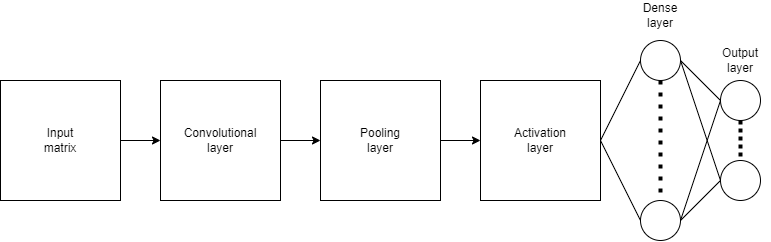
\includegraphics[width=\textwidth]{dependencies/pictures/CNN_example.png}
        \caption{Convolutional neural network example.}
        \label{fig:cnn-example}
    \end{figure}

    \subsubsection*{Convolutional layer}\label{sec:convolutional-layer}
    As it was mentioned before, convolutional layer is capable of detecting patterns (features) such as edges on given input picture. This process can be done with use of filters (also known as kernels). Kernels are small matrices containing numbers which also are modifiable parameters used in learning process. Each  convolution layer consists of some number of kernels from which each of them is used to detect some kind of pattern. For example, to recognize hand-written $1$, two kernels can be used. First for detecting diagonal line and second one to detect straight line.

    To check if given pattern exist in input data, each convolution layer perform \textbf{Cross-correlation} operation on input data and all kernels. Cross-correlation can be performed by ,,sliding'' given kernel matrix over input data and computing \textbf{Frobenius inner product} (summing calculated element-wise multiplication products) \cite{bib:book-frobenius-inner-product} for all intersections. That calculated values creates output matrix of the cross-correlation operation. Mathematical equation for cross correlation can be written as follows:
    \begin{equation}
        G[i, j] = \sum_{u = 0}^{l} \sum_{v = 0}^{k} h[u, v] F[i+u. j+v],
    \end{equation}
    \begin{equation}
        G = h \bigotimes F,
    \end{equation}
    where:
    \begin{itemize}[label=]
        \item $G[i, j]$ -- output matrix value of indexes $i$ and $j$, $l$ -- size of the input matrix, $k$ -- size of the kernel, $h$ -- kernel, $F$ -- input matrix \cite{bib:article-cross-correlation}.
    \end{itemize}
    Example of cross-correlation operation can be seen on \hyperref[fig:cross-correlation-example]{fig. \ref*{fig:cross-correlation-example}}.
    \begin{figure}
        \centering
        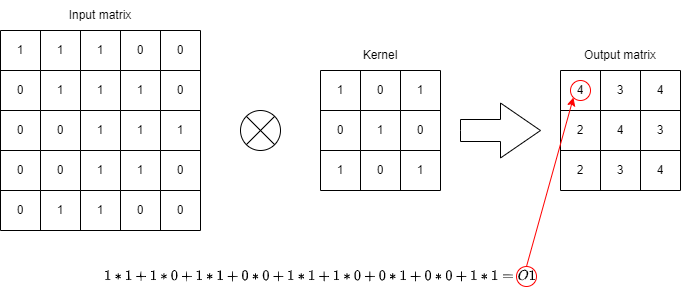
\includegraphics[width=\textwidth]{dependencies/pictures/Cross-correlation_example.png}
        \caption{Cross-correlation example.}
        \label{fig:cross-correlation-example}
    \end{figure}
    Important thing to mention is the fact that cross-correlation operation can be performed with different \textbf{stride} (size of the step with which kernel is sliding over input matrix). The most common stride to use is $1$ but it can be changed. In case of this thesis, all cross-correlation operations are performed with stride of $1$. It is possible to calculate size of cross-correlation output matrix by using equation:
    \begin{equation}
        n_{out} = floor((l - k) / s) + 1,
    \end{equation}
    where:
    \begin{itemize}[label=]
        \item $n_{out}$ -- size of output matrix, $l$ -- size of the input matrix, $k$ -- size of the kernel, $s$ -- stride.
    \end{itemize}

    In each convolutional layer first think that is performed on input data is a cross-correlation between input matrix and all the kernels that the layer consists of. Important thing to mention is the fact that the output of the convolutional layer can be different. Number of matrices produced by layer is determine by number of kernels inside that layer. After performing cross-correlation operation, to each output matrix is added bias matrix \cite{bib:internet-aa-cnn-lecture}. In conclusion, output of convolutional layer with one kernel can be described by equation:
    \begin{equation}
        Conv_{out} = h \bigotimes F + B,
    \end{equation}
    where:
    \begin{itemize}[label=]
        \item $Conv_{out}$ -- convolutional layer output matrix, $h$ -- kernel, $F$ -- input matrix, $B$ -- bias matrix.
    \end{itemize}

    \subsubsection*{Pooling layer}\label{sec:pooling-layer}
    Pooling layer is the second distinctive element of convolutional neural network. As it was mentioned before, main purpure of pooling layer is to reduce size of the matrix that is used for calculations. There are a lot of possible functions that can be performed in this layer but two the most common are \textbf{Max Pooling} and \textbf{Average Pooling} \cite{bib:book-pooling-methods}. In case of this thesis, Max Pooling method has been used. 

    Max pooling method is also used to highlight the most important parts of the feature map. This operation works in the similar way to cross-correlation operation. Each pooling layer consists of window of the specific size which slide over input matrix, with specific stride (similar like in cross-correlation operation). While sliding over input matrix, algorithm pick maximal value and pass it into output matrix. Max pooling example can be seen on \hyperref[fig:max-pooling-example]{fig. \ref*{fig:max-pooling-example}}
    \begin{figure}
        \centering
        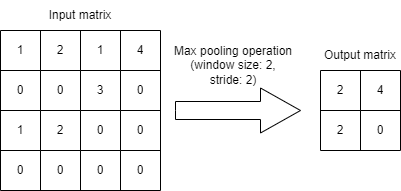
\includegraphics[width=\textwidth]{dependencies/pictures/Max_Pooling_example.png}
        \caption{Max pooling example.}
        \label{fig:max-pooling-example}
    \end{figure}

    \subsection{Learning process for neural network instance}\label{sec:learning-process-for-nn-instance}
    After describing two types of neural network that will be used in following thesis, last thing that needs to be explained is learning process. This process looks similar in both neural networks (ANN and CNN) so it will bee described as one. When neural network is created, values of all weights and biases are set randomly and that will result in network answers also being random \cite{bib:article-how-neural-network-learn}. To make network answers more sensible it needs to be ,,taught'' how to approach the problem. Method of machine learning that will be used to improve neural network answers is called \textbf{supervised learning}. This type of learning method is based on examples and target output. Dataset that is used for training needs to have input data and target data to calculate how ,,bad'' was model answer \cite{bib:book-statistical-learning}. Learning process consists in periodic algorithm which will result in updating values of weights and biases. This process begins with splitting data set into two sets (training set and test set). Next, each example of training set need to be inputted into model and output needs to be read. When model output will be acquired it needs to be compared with target data for given example. One of the methods of performing this comparison is to calculate \textbf{loss function}. This is place is the first one in which learning process for ANN and CNN is slightly different. For both models loss function will be calculated, but formula for calculating this function will be different in each type of network. Loss function for artificial neural network will be calculated using formula:
    \begin{equation}
        \lambda_{ANN} = t - ANN_{out},
    \end{equation}
    where:
    \begin{itemize}[label=]
        \item $\lambda_{ANN}$ -- value of loss function for artificial neural network, $t$ -- target value for given example, $ANN_{out}$ -- output of the model.
    \end{itemize}
    Loss function for convolutional neural network will be calculated using formula:
    \begin{equation}
        \lambda_{CNN} = -\sum t \log CNN_{out},
    \end{equation}
    where:
    \begin{itemize}[label=]
        \item $\lambda_{CNN}$ -- value of loss function for convolutional neural network, $t$ -- target value for given example, $CNN_{out}$ -- output of the model.
    \end{itemize}
    By calculating loss functions for both models, it is possible to check how incompatible models answers are from desirable output. 

    Unfortunately, knowing how bad specific model performs in given task, won't result in making it better. To improve performance of given model, \textbf{Backpropagation algorithm} can be used \cite{bib:book-make-own-neural-network,bib:internet-convolutions-and-backpropagation}. Backpropagation algorithm is the most important component in whole learning process because this methodology allows for improving how model perform. Main idea of this algorithm is backward propagation of computed error (loss function), which is based on calculating \textbf{gradient} value for given loss function ($\nabla f$). Result of this operation is the set of values which shows how values of output layer should change to decrease loss function. Unfortunately, there is no possibility to change neurons values directly. There is possibility to impact neuron value by modifying following components: 
    \begin{itemize}
        \item values of input weights,
        \item value of biases,
        \item values of neurons in previous layer.
    \end{itemize}
    The same methodology can be applied to all layers in the network. Last important thing, worth mentioning, is the fact that learning process for both ANN and CNN looks the same but equations, used for calculating gradient are different for each network type.

    In conclusion, learning process of neural network model can be described by 5 steps:
    \begin{enumerate}
        \item Load training data into model,
        \item Using feedforward algorithm obtain output of the model,
        \item Calculate loss function for given example,
        \item Using backpropagation algorithm, calculate gradient values for all weights and biases,
        \item Update values of all weights and biases.
    \end{enumerate}
    After processing all examples from training set, test set is used to check model accuracy. If accuracy is to low, it is necessary to repeat training process. This sequence of action can be repeated until obtained accuracy will be acceptable (potentially, global minimum of the loss function will be achieved) \cite{bib:internet-aa-cnn-lecture,bib:book-make-own-neural-network}. To improve, obtained results and to increase probability of finding global minimum of the loss function, there is 1 modification of backpropagation algorithm that will be used in scope of this thesis. There is parameter called \textbf{learning rate} \cite{bib:internet-learning-rate}. This is value which define how big changes will be applied to weights and biases. Because final goal of the backpropagation algorithm is finding global minimum of the loss function, if the changes will be to big, it can result in constant passing the proper minimum value. Usage of proper learning rate value reduce probability of it happening.

    \section{Other approaches to the problem}\label{sec:other-approaches-to-problem}
    After describing problem approach that will be used in scope of this thesis, it is important to mention what other solutions to the Chess AI problem can be found. First approach is very similar to described solution because it uses all mentioned components except of neural network instance. This solution assumes usage of complex mathematical equations to evaluate chessboard situation. This type of approach is caller \textbf{heuristic approach} \cite{bib:article-computer-chess-move-ordering,bib:internet-step-by-step-chess-ai}. The main problem of heuristic approach is the fact that this solution is very time consuming and require big knowledge of chess game to implement correctly. Another disadvantage of this approach is the fact that it is very linear solution and it is hard to implement some unpredictability which can result in small effectivity against more advanced chess players.

    Second possible approach looks much more promising but it is also much harder to implement. This approach assumes usage of self-improving neural network. Mentioned before AlphaZero software uses this exact method for playing \cite{bib:internet-alphazero}. Basic idea behind this approach is to create some kind of algorithm which will be building and modifying neural network structure while playing with real opponent. This method is very popular and very efficient in game theory because it can result in creating ,,unbeatable'' AI. Main advantage of this solution is the fact that the more games will be played by AI instance, the smartest it gets \cite{bib:article-self-improving-nn}. Usage of this method can result in very interesting results but it is also very hard to implement. Another problem regarding this solution is time consumption and quality of ,,training resources''. If created AI will play with the best players, it will learn a lot but in the other case it can stop improving.

% References to 
% book \cite{bib:book},
% scientific papers in journals \cite{bib:article},
% conference papers \cite{bib:conference},
% and web pages \cite{bib:internet}.

% Equations should be numbered:
% \begin{align}
% y = \frac{\partial x}{\partial t}
% \end{align}

%\chapter{[Problem analysis]}
%
%\begin{itemize}
%\item problem analysis, problem statement
%\item state of the art, literature research (all sources in the thesis have to be referenced, eg journal article \cite{bib:article} book \cite{bib:book}, conference paper \cite{bib:conference}, internet source \cite{bib:internet})
%\item description of known solutions, algorithms
%\item location of the thesis in scientific domain
%\item The title of this chapter is similar to the title of the thesis.
%\end{itemize}
